\documentclass[12pt,a4paper, french]{report}

% ================================
%            PACKAGES
% ================================

\usepackage[T1]{fontenc}
\usepackage[utf8]{inputenc}
\usepackage[french,english]{babel}
\usepackage{xcolor}
\usepackage{graphicx}
\usepackage{fancyhdr}
\usepackage{amsmath}
\usepackage{eso-pic}
\usepackage{leftidx}
\usepackage{float}
\usepackage{lastpage}
\usepackage{appendix}
\usepackage{caption}
\usepackage[colorlinks=true,
            urlcolor=black,
            linkcolor=black,
            breaklinks=true,
            citecolor= black,
            plainpages=false
            ]{hyperref}

% ================================
%             MARGIN
% ================================

\setlength{\topmargin}{-20mm}
\setlength{\oddsidemargin}{10mm}
\setlength{\evensidemargin}{10mm}
\setlength{\textwidth}{140mm}
\setlength{\textheight}{250mm}

% ================================
%            SETTINGS
% ================================

\pagestyle{fancy}
\fancyhf{}
\renewcommand{\headrulewidth}{0pt}
\fancyfoot[C]{\textbf{page \thepage~sur~\pageref{LastPage}}}

\fancypagestyle{plain}{%
    \fancyhf{}
    \fancyfoot[C]{\textbf{page \thepage~sur~\pageref{LastPage}}}
}

% ================================
%            COMMANDS
% ================================

\newcommand{\itemstitle}[1]{\centering{\LARGE #1}\vskip1cm}
\newcommand{\sectitle}[1]{\frame{\huge#1\\\hrulefill}}
\newcommand{\code}[1]{\texttt{#1}}
\newcommand{\acro}[1]{\MakeUppercase{#1}}
\newcommand{\citer}[1]{\og #1 \fg}
\newcommand{\propre}[1]{\textsc{#1}}
\newcommand{\nom}[2]{\textrm{#1} \textsc{#2}}
\newcommand{\soc}[1]{\texttt{#1}}
\newcommand{\auto}{{\color{automatica-blue}\tahomab automatica}}
\newcommand{\labo}{\texttt{\propre{Labosoft}}}
\newcommand{\cali}{\texttt{\propre{Calisoft}}}
\newcommand{\windev}{\texttt{WINDEV}}
\newcommand{\wlang}{\texttt{\propre{WLangage}}}
\newcommand{\excel}{\texttt{\propre{Excel}}}
\newcommand{\ofni}{\textbf{\textcolor{coderedpink}{O}\textcolor{codecyan}{F}\textcolor{codeorange}{N}\textcolor{codegreen}{I}}}


% ================================
%           REPORT INFO
% ================================

\title{\LARGE{Rapport de projet tutoré}\\[0,5cm] % Titre
        \textbf{\Huge{Refonte d'un site internet}}\\[0,1cm]
        \textbf{\Huge{pour une association étudiante}}}
\author{\Large{\nom{Tristan}{Amiotte-Suchet}}\\
        \Large{\nom{Antoine}{Cuinet}}\\[0,2cm]
        \Large{\nom{Gaspard}{Quentin}}}
\date{Février 2025}

% ================================
%             DOCUMENT
% ================================

\begin{document}
\selectlanguage{french}
\hypersetup{pdfborder=0 0 0}

\makeatletter
\begin{titlepage}
  \enlargethispage{3cm}

  \AddToShipoutPictureBG{
        \put(45,730){\includegraphics[width=6cm]{assets/pictures/logo_ufc.png}}
    }

  \begin{center}
    \vspace*{4,4cm}
    \textsc{\@title} \\
    \vspace*{0,3cm}
    \HRule%
    \vspace*{0,3cm}
    \large{\@author} \\
    \vspace*{1cm}
    \anneeUniversitaire
    \vspace*{1,2cm}
    \includegraphics[width=12cm]{assets/pictures/home-page.png}\\
    \vspace*{0cm}
  \end{center}

  \vspace*{1cm}
  \noindent
  \normalsize{\strong{Tuteurs de projet:} \nom{Alexandre}{Demougin}  \& \nom{Alicia}{Pierrot}}\\
  \vspace*{0.5cm}

  \noindent
  \normalsize{\strong{Établissement de formation:} \textsc{\univ}}\\

\end{titlepage}
\ClearShipoutPicture
\thispagestyle{empty}
\setcounter{page}{0}
\null
\newpage

\chapter*{Remerciements}

Nous tenons tout d'abord à remercier nos tuteurs de projet pour leur soutien et leur encadrement, Monsieur \nom{Alexandre}{Demougin} et Madame \nom{Alicia}{Pierrot}, qui nous ont guidés tout au long de ce projet. 
Leurs précieuses indications et conseils ont été d'une grande aide pour la réalisation du projet.
\bigskip

Nous remercions également l'\univ, et plus particulièrement le département d'informatique, qui, de par ses enseignements, nous a transmis les savoirs et les compétences nécessaires à la réalisation de ce projet.
\bigskip


Enfin, nous remercions également les étudiants testeurs, qui nous ont fait part de leurs retours sur le site que nous avons produit.

\cleardoublepage
% \Large
\tableofcontents
\listoffigures
% \listofalgorithms
\normalsize
\chapter*{Glossaire}
\label{chap:glossary}

\begin{description}
    \item[CMS] Un système de gestion de contenu (\langue{Content Management System}) est un logiciel qui permet de créer, modifier et publier du contenu sur un site \web.
    \item[CAS] Le \langue{Central Authentication Service} est un système d'authentification centralisé permettant à un utilisateur de se connecter à plusieurs services avec un seul identifiant.
    \item[RGPD] Le \citer{Règlement Général sur la Protection des Données} est un règlement de l'Union Européenne qui encadre le traitement des données personnelles.
    \item[Regex] Une expression régulière (\langue{Regular Expression}) est une chaîne de caractères qui décrit un ensemble de chaînes de caractères possibles selon une syntaxe précise.
\end{description}

\noindent\HRule
\vspace{1cm}

\Large\noindent \strong{Terminologie spécifique au site de l'\ofni}\normalsize

\begin{description}
    \item[Instance d'événement] Une occurrence d'un événement, c'est-à-dire une édition précise de ce dernier.
    \item[Form-Widget] Un ensemble de champs de formulaire qui peuvent être réutilisés pour créer des formulaires plus complexes. Il en existe trois types~: \code{natif}, \code{composite} et \code{liste}.
\end{description}

\chapter{Introduction}
\label{chap:intro}

Dans le cadre de notre troisième année de Licence Informatique à l’\univ\~ de \propre{Besançon}, nous avons eu l’opportunité de réaliser un projet tutoré en équipe. Ce projet a pour objectif de concevoir et développer un nouveau site \web\ pour l’\ofni, l’association des étudiants en informatique de notre université.
\bigskip

L’objectif principal de ce projet est d’appliquer nos connaissances en développement \web\ tout en en acquérant de nouvelles. Il s’agit non seulement de produire un site fonctionnel et maintenable, mais également d’adopter une méthodologie rigoureuse, de la conception jusqu’au déploiement de celui-ci.
\bigskip

Encadrés par nos tuteurs, Monsieur \nom{Alexandre}{Demougin}, doctorant au département informatique de l'Université, et Madame \nom{Alicia}{Pierrot}, gestionnaire administrative et financière, nous avons ainsi suivi un processus structuré comprenant l’analyse des besoins, le maquettage, le choix des technologies et l’implémentation des différentes fonctionnalités.
\bigskip

Ce rapport vise à détailler les différentes étapes du projet, en mettant en avant les choix techniques effectués, les difficultés rencontrées ainsi que les perspectives d’amélioration du site.

\chapter{Le site web de l'associassion \ofni}
\label{chap:site}

Le but de ce projet est de réaliser le site internet de l'association \ofni.

\section{L'\ofni}
\label{sec:ofni}

Fondée en 1997, l'\ofni\ est l'association des étudiants en informatique de l'\univ\ de \propre{Besançon}.
\bigskip

L'association a pour but de réunir les étudiants des différentes promotions autour d'activités communes (sorties, barbecue, nuit de l'info\ldots) et de permettre une entraide entre promotions.
\bigskip

L'\ofni\ fait également office d’intermédiaire entre les membres de l’association, les chercheurs et les entreprises en conservant un réseau d’anciens membres et des contacts avec nos sponsors.

\section{Présentation du projet}
\label{sec:presentation-projet}

Ce rapport présente le développement que nous avons réalisé dans le câdre du projet tutoré de troisième année de Licence Informatique au sein de l'\univ.
\bigskip

Le sujet de ce projet est de développer un site \web\ pour une association étudiante, en équipe de 2 ou 3 personnes.
Le tout dans l'objectif de mobiliser nos compétences en développement \web\ et d’en acquérir de nouvelles.
Nous avons pour cela été encadrés par M. \nom{Alexandre}{Demougin} et par Mme. \nom{Alicia}{Pierrot}, de la conception à la mise en ligne du site, ainsi que pour la réalisation de ce rapport et de notre soutenance orale.

\section{Objectifs du site}
\label{sec:objectifs-site}

Les consignes sur la réalisation du site étaient de créer une interface claire et intuitive, de développer une solution robuste et fonctionnelle, le tout en mettant l’accent sur l’efficacité et la maintenabilité du site.
\bigskip

Les pistes de fonctionnalités proposées étaient de présenter les diverses activités réalisées par l’association, que le site serve de vitrine pour les projets des étudiants, qu'il permette la réalisation de sondages pour un événement et de pouvoir fournir des informations aux lycéens souhaitant découvrir cette association.

\section{Plan de réalisation du projet}
\label{sec:plan-realisation}

Nous avons eu quelques mois, en parallèle de nos études pour mener à bien ce projet. Celui-ci était divisé en deux grandes phases.
\bigskip

La première, de novembre à décembre 2024, portait sur la phase de conception et de maquettage du site. Celle-ci consistait dans un premier temps à trouver les fonctionnalités du site ainsi que les besoins auxquels il devait répondre. Dans un second temps, cette phase consistait en l'élaboration de la maquette du site, contenant l'entièreté des pages du site ainsi que leurs visuels.
\bigskip

La seconde étape, de janvier à février, était la phase de développement du site. Celle-ci correspond à une période de recherche et de réflexion sur les technologies existantes et le choix des plus adaptées pour la réalisation du projet, ainsi que le développement et le codage du site.

\chapter{Le développement du nouveau site}
\label{chap:dev}

% Ne pas lire pour l'instant !!

% TODO: Peut-être revoir où placer la partie répartition du travail, vu qu'on annonce ce qui a été fait par qui, alors que l'on n'a pas encore annoncé ce que l'on voulait faire et ce qui a été implémenté.

% TODO: Peut-être restructurer et mettre la répartition du travail comme une sous-section en début de chaque partie (maquette, développement).

Lors de la première phase du projet, nous avons tout d'abord dû réfléchir aux besoins auxquels le site devait répondre.
À travers plusieurs réunions, nous avons alors réfléchi aux améliorations que nous souhaitions apporter par rapport à l’ancien site de \ofni\ et défini la liste des fonctionnalités que nous souhaitions implémenter.

C'est également à ce moment-là que nous avons dû juger de la faisabilité de certaines fonctionnalités au regard du \logo{RGPD} (Règlement Général sur la Protection des Données).

\subsection{Fonctionnalités du site}
\label{subsec:fonctionnalites}

Ainsi, après ces réunions, voici les fonctionnalités principales que nous avons retenues :

\begin{itemize}
    \item Une page de présentation de l'association et de son histoire
    \item Une page événements et la possibilité de s'inscrire à ces derniers
    \item Une page actualités
    \item Une page boutique permettant d'acheter des produits et d'adhérer à l'association
    \item Une page galerie photos
    \item Un jeu (ajouté au cours de la phase de développement du projet)
    \item Un formulaire de contact pour les entreprises
    \item Une page administrateur pour les futurs bureaux de l'\ofni\ afin de simplifier la transmission de l'association
    \item Un compte utilisateur permettant :
    \begin{itemize}
        \item d'accéder à la galerie photos,
        \item d'accéder au jeu,
        \item de s'inscrire aux événements et de les gérer.
    \end{itemize}
    \item Un compte administrateur permettant :
    \begin{itemize}
        \item de gérer les événements et les actualités,
        \item de gérer les photos,
        \item d'accéder à la page administrateur.
    \end{itemize}
\end{itemize}

\section{Le maquettage du nouveau site}
\label{sec:maquettage}

% TODO: Ajouter des images pour illustrer la maquette.

Une fois ces fonctionnalités définies, nous avons entamé la conception de la maquette du site en deux étapes. Une première version manuscrite nous a permis de structurer le site de manière schématique, puis une version finalisée a été réalisée sur \logo{Figma} afin d’obtenir une maquette propre et exploitable.

L'objectif principal de cette maquette était de confirmer les fonctionnalités désirées et de commencer à visualiser leur implémentation et la forme qu'elles allaient prendre, sans se concentrer sur la charte graphique ni sur le design visuel du site.

\subsection{Version manuscrite}
\label{subsec:maquette-manuscrite}

Dans un premier temps, nous avons réalisé une esquisse manuscrite afin d’organiser les différentes pages du site et de positionner les éléments fonctionnels. Cette étape a été cruciale dans ce projet puisqu'elle nous a facilité la réflexion sur la structure générale du site et l'agencement des fonctionnalités.

C'est également ici que nous avons commencé à imaginer comment rendre notre site le plus maintenable possible sans ajouter de code supplémentaire. Nous avons pensé à créer la possibilité de gérer le contenu du site sans code (comme le ferait un système de gestion de contenu comme \logo{Wordpress} par exemple)
Nous avons également imaginé et schématisé un système de génération de formulaires personnalisés pour les événements.


\begin{figure}[H]
    \centering
    \includegraphics[scale=0.5]{assets/pictures/maquette-inscription.pdf}
    \captionsetup{justification=centering}
    \caption{Page de la maquette manuscrite concernant le système d'inscription à des événements}
    \label{fig:maquette-inscription}
\end{figure}


Une fois cette version manuscrite terminée, nous avons échangé avec nos tuteurs afin d’ajuster certains éléments.
Nous avons notamment été amenés à repenser la façon dont l'utilisateur devait interagir avec le site afin de rendre l'expérience la plus intuitive possible.

\subsection{Version finalisée sur \logo{Figma}}
\label{subsec:maquette-figma}

Après plusieurs ajustements, nous
avons commencé l'élaboration d'une version numérique finalisée sur l'outil \logo{Figma}.
Bien que nous ne connaissions pas le logiciel, nous avons pu rapidement le prendre en main et il nous a ainsi permis de transformer nos brouillons manuscrits en une maquette plus aboutie et fidèle à notre vision du projet.

\begin{figure}[H]
    \centering
    \includegraphics[scale=0.4]{assets/pictures/figma.png}
    \caption{Quelques pages de la maquette numérisée}
    \label{fig:maquette-figma}
\end{figure}

De plus l'apprentissage de \logo{Figma} a également permis à Antoine, qui était chargé du design et de la charte graphique du site, de pouvoir effectuer des maquettes stylisées afin de trouver le visuel qu'il souhaitait appliquer au projet.

\section{Les technologies utilisées}
\label{sec:technologies-utilisees}

Une fois la maquette finalisée, nous avons sélectionné les technologies les plus adaptées pour développer un site performant et facilement maintenable par les futurs membres de l’association.

\subsection{Le \langue{framework} \logo{Symfony}}
\label{subsec:symfony}

Pour le développement du serveur, nous avons choisi un \langue{framework} \logo{PHP}, ayant déjà appris ce langage lors de l’unité d’enseignement \citer{Langages du Web} en deuxième année de licence. Ce choix nous permettait de nous concentrer sur l’architecture du projet sans devoir apprendre un nouveau langage, tout en assurant une continuité pour les futurs membres de l’association qui connaîtront également \logo{PHP}.

Après avoir comparé \logo{Laravel} et \logo{Symfony}, nous avons opté pour ce dernier, son architecture orientée objet étant plus familière et mieux adaptée à notre approche du développement.

\subsection{Le moteur de \langue{template} \logo{Twig}}
\label{subsec:twig}

Pour générer dynamiquement les pages \logo{HTML}, nous avons utilisé \logo{Twig}, le moteur de \langue{template} recommandé par \logo{Symfony}. Ce choix a facilité la séparation entre la logique métier et l'affichage, améliorant ainsi la lisibilité et la maintenabilité du code.

\subsection{Le langage \logo{JavaScript}}
\label{subsec:javascript}

En cours de projet, nous avons été amenés à ajouter une nouvelle fonctionnalité au site : un jeu ludique ayant pour objectif de donner envie aux étudiants de venir sur le site de façon régulière.
L'idée nous a été proposée par un de nos tuteurs, M. \propre{Demougin}, après la conception de la maquette \logo{Figma}.
Cette idée nous a beaucoup plu, et nous avons alors décidé d'implémenter une version revisitée du célèbre jeu \logo{Space Invaders}.

Le langage \logo{JavaScript} a été rapidement adopté pour la réalisation de cette partie du projet, en raison de son intégration facile et de sa compatibilité avec la grande majorité des navigateurs.

\subsection{Le préprocesseur \logo{Sass}}
\label{subsec:sass}

Afin d’améliorer la structuration et la maintenabilité du code \logo{CSS}, nous avons utilisé le préprocesseur \logo{Sass}. Cet outil a permis une meilleure organisation des styles et une gestion plus efficace de la mise en page, garantissant une adaptation optimale du site à tous types d’écrans. L’utilisation de \logo{Sass} facilitera également d’éventuelles évolutions graphiques du site dans le futur.

\section{Répartition du travail}
\label{sec:repartition-travail}

Afin de travailler efficacement en groupe, nous avons réparti la charge de travail de manière équilibrée entre les membres de l'équipe.

Pour la conception de la maquette, nous avons d'abord réfléchi ensemble aux différentes pages qui devaient composer le site, avant que chacun ne prenne en charge certaines d’entre elles. Cette répartition s’est faite naturellement, chacun ayant des préférences différentes.

Lors de la phase de développement, et sur les conseils de nos tuteurs, M. \propre{Demougin} et Mme. \propre{Pierrot}, nous avons adopté l’outil \logo{Trello}. Cet outil nous a permis de lister et d’organiser les différentes tâches à accomplir, tout en suivant leur état d'avancement. En collaboration avec nos tuteurs, nous avons ainsi identifié les fonctionnalités à implémenter et avons réparti leur développement au sein du groupe.

Antoine a pris en charge l’implémentation du front-end du site ainsi que le développement du jeu. Il a également rédigé la majorité des contenus textuels du site.
Tristan s’est occupé de l’implémentation du système d’ajout et de gestion dynamique des événements et des articles, ainsi que de la création des formulaires d’inscription aux événements. Il a également développé la page boutique.
Gaspard s’est quant à lui chargé de la mise en place du système d’authentification et de gestion des comptes, ainsi que de la dynamisation de certaines pages, notamment celles dédiées au jeu et à la présentation de l’association. Il a également développé les formulaires de contact, le système d’envoi automatisé d’\langue{e-mails} et la page galerie photos.

\section{Les difficultés rencontrées}
\label{sec:difficultes}

Plus concrètement, l'implémentation du site se voit confrontée à plusieurs difficultés et interrogations, tant techniques qu'éthiques. Il est attendu de la partie CMS du site, une certaine factorisation. Mais le stockage des données personnelles ainsi que la décision d'autoriser ou non une inscription, sont des questions qui sont à prendre en compte du début à la fin du développement.

\subsection{L'autorisation d'inscrition}
\label{subsec:autorisation-inscription}

Qui peut profiter, et donc s'inscrire, aux événements de l'\ofni~? Ce sont les personnes qui possèdent un compte sur le site internet. Mais la même question revient alors, qui peut créer un compte~? Une décision s'impose alors rapidement~: toute personne membre de l'\univ\ peut se créer un compte, ainsi que certaines autres personnes, comme des alumni par exemple, mais uniquement sur autorisation manuelle du bureau de l'association.

Il faut alors trouver un élément concret qui permet de distinguer un membre de l'\univ\ d'une autre personne. Il est alors logique de se tourner vers les adresses e-mails. En effet, les adresses e-mails des membres de l'\univ\ sont de la forme~: \code{prenom.nom@[edu.]univ-fcomte.fr}.

Lors de la réception d'une nouvelle demande d'inscription, l'algorithme doit donc simplement vérifier que l'adresse \langue{e-mail} de la personne soit conforme au spécimen précédent. Si c'est le cas, alors l'inscription est automatiquement validée à compter de l'instant ou la personne aura utilisé le lien de confirmation d'adresse qui lui a alors été envoyé. Sinon, il doit en faire manuellement la demande via le formulaire de contact situé sur la page d'accueil du site. Qu'importe la voie utilisée, une fois le compte créé, l'utilisateur peut alors s'inscrire aux différents événements.

\subsection{La génération de formulaire}
\label{subsec:generation-formulaire}

L'inscription à un événement nécessite, dans la quasi totalité des cas, le remplissage d'un formulaire par l'utilisateur. Ce dernier étant susceptible de changer à chaque événement, il est donc nécessaire de pouvoir générer dynamiquement ces formulaires en fonction des besoins. Pour cela, l'idée est alors de stocker les formulaires dans la base de données au format \logo{JSON}. Ainsi, lors de la création d'un événement, l'organisateur peut définir le formulaire qui doit être utilisé pour l'inscription. Si ce formulaire n'existe pas déjà, il peut alors le créer. Puis, lors de l'inscription, l'affichage du formulaire côté utilisateur est généré automatiquement en fonction des données stockées.

\subsection{La factorisation des événements}
\label{subsec:factorisation-evenements}

Avoir des formulaires réutilisables est un grand atout pour l'aspect \logo{CMS} du site. Mais au delà de l'inscription, la page utilisée pour présenter chaque événements, rique d'être très similaire d'année en année sur deux éditions d'un même événement. Il est alors nécessaire de pouvoir factoriser ces pages pour éviter de devoir tout recréer tous les texts et toutes les illustrations.
\bigskip

Pour pallier à ce souci de factorisation, la structure du site permet alors à l'administrateur de créer d'abord un événement. Ce dernier est intemporel et n'est donc pas lié à une édition spécifique. Ce dernier centralise un nom, une illustration ainsi qu'un texte de présentation puis un autre texte de résumé. Dans un deuxième temps, l'administrateur peut alors créer une édition de cet événement. Cette édition est alors liée à l'événement et contient les informations spécifiques à son déroulement, comme la date, le lieu, le prix, etc. Ceci est, dans la terminologie du site, appelé une \citer{Instance d'événement}, faisant ainsi une petite référence au monde du développement, qui est après tout le point commun de tous les membres de l'\ofni.

Pour ce qui est de la page qui présente chaque édition d'un événement et fournit le lien d'inscription, elle est alors générée automatiquement à partir des données de l'instance d'événement.

\chapter{Le travail réalisé}
\label{chap:travail-realise}

Le développement du site achevé permet alors de voir avec un peu plus de recul ce qui a concrètement été réalisé, rajouté ou abandonné. Tout cela permet également une comparaison avec les objectifs initiaux du projet donnés en grande partie par la maquette du site.

\section{Ce qui a été implémenté}
\label{sec:implem}

Regardons d'abord ce qui est fonctionnel à l'heure où le site se voit mis en ligne pour la première fois.

\subsection{Les pages de formalités}
\label{subsec:pages-formalites}

% home page screenshot
\begin{figure}[h]
    \centering
    \includegraphics[width=\textwidth]{assets/pictures/home-page.png}
    \caption{Page d'accueil du site de l'\ofni}
    \label{fig:home-page}
\end{figure}

Le site contient un certain nombre de pages de formalités, qui sont des pages statiques pour la plupart. On y trouve notamment l'accueil du site, que l'on peut voir \figureref{fig:home-page}, la page de présentation de l'association, celle d'adhésion ainsi que celle des mentions légales. Certaines de ces pages sont présentent des informations qu'il est, juridiquement, obligatoire de faire apparaître sur un site web. C'est le cas des mentions légales, qui sont des informations sur l'association, son siège social, son numéro de téléphone, son adresse \langue{e-mail}, son numéro de \logo{SIRET}, etc.

Il est tout de même possible de trouver un petit peu de dynamisme sur certaines pages, notamment la page d'accueil qui contient des petits \langue{teasers} sur les activités à venir de l'association, ou encore des actualités.

\subsection{Le jeu \game}
\label{subsec:jeu}

% game screenshot
\begin{figure}[h]
    \centering
    \includegraphics[width=\textwidth]{assets/pictures/game.png}
    \caption{Vue du jeu \game}
    \label{fig:game}
\end{figure}

Peu avant le début de la phase de développement, il fut décider d'ajouter un petit jeu vidéo au site avec un afficage du meilleur joueur pour rendre la visite du site plus attractive. Le jeu \game\ est un jeu de type \citer{Space Invaders} où le joueur doit tirer sur des vaisseaux ennemis pour marquer des points. Le jeu est jouable directement depuis le site, sans avoir besoin de télécharger quoi que ce soit. On peut voir une capture d'écran du jeu \game\ en \figureref{fig:game}.

\subsection{La connexion et l'inscription aux événements}
\label{subsec:connexion-inscription}

Ces actualités et événements de l'\ofni\ constitue la partie centrale du site. Tout cela commence évidemment par un page de connexion, ou de création de compte si l'utilisateur n'en a pas encore. Une fois connecté, l'utilisateur peut alors s'inscrire à des événements.

Comme vu dans la section \ref{subsec:generation-formulaire}, les formulaires d'inscription aux événements sont générés automatiquement à partir des informations de la base de données. Cela permet de ne pas avoir à modifier le code du site à chaque nouvel événement ou bien de réutiliser un même formulaire pour plusieurs éditions.
\bigskip

Lorsque l'administrateur décide de créer un nouveau formulaire, il va en réalité définir ce qui, dans la terminologie du présent site, s'appelle un \formwidget. Il existe trois types de \formwidget\ différents~:
\begin{description}
    \item[Natif] Qui correspond à un champ simple, comme par exemple un texte, une date, ou encore une case à cocher. Ils sont définis par défaut dans le site et ne peuvent pas être modifiés ou ajoutés par l'administrateur. Ils sont les briques fondamentales pour la construction d'autres \formwidget\ plus avancés.
    \item[Composite] Un ensemble de \formwidget\ les uns à la suite des autres. Par exemple, un \formwidget\ composite pourrait être un \formwidget\ natif de type text, suivi d'un \formwidget\ natif de type date, puis d'un autre \formwidget\ composite défini en amont. Ils sont définis par l'administrateur et peuvent être réutilisés dans d'autres \formwidget.
    \item[Liste] Un ensemble de taille indéfinie de \formwidget\ de même type, mais qui peuvent être répétés autant de fois que nécessaire. Par exemple, un \formwidget\ liste pourrait être un \formwidget\ composite décrivant un membre d'une équipe ; l'utilisateur peut alors, lors de son inscription, en remplir autant de fois qu'il ne le faut pour que tous les membres du groupe soient enregistrés. Ils sont définis par l'administrateur et peuvent être réutilisés dans d'autres \formwidget.
\end{description}

Lorsque l'utilisateur s'inscrit à un événement, le formulaire, correspondant à un \formwidget, est alors généré dynamiquement. Il est alors possible de définir des formulaires très complexes, avec des champs de différents types, des champs répétables, etc.

\section{Ce qui n'a pas été implémenté}
\label{sec:non-implem}

Il est important de noter que tout n'a pas été implémenté. Les différentes réunions de travail ont permis de définir les priorités et de déterminer ce qui était le plus important pour le site. Certaines fonctionnalités ont alors été retirées pour cause d'une utilité moindre ou d'une impossibilité à les commencer, tandis que d'autres ont été ajoutées en cours de développement.
\bigskip

On peut par exemple noter qu'au départ, il fut prévu que le système de connexion passe par le \logo{CAS} officiel de l'\univ. Cependant, les demandes d'autorisation pour utiliser ces systèmes n'ayant pas abouti, l'idée a dû finalement être abandonnée. Il en est de même pour la gestion des utilisateurs, qui devait être faite par le \logo{CAS}.

Mais au-delà des restrictions administratives, d'autres fonctionnalités n'ont pas vu le jour par pure manque de temps. C'est par exemple le cas du \citer{Crochet \logo{Discord}}, qui devait permettre de diffuser automatiquement les événements de l'\ofni\ sur le serveur \logo{Discord} de l'association dès la création de l'événement sur le site.

\section{Projection pour l'avenir}
\label{sec:avenir}

Certes, tout n'est pas implémenté. À ce jour, le site est fonctionnel et permet de remplir les objectifs principaux qui lui ont été fixés. Ajoutant en plus certaines fonctionnalités comme \game. Il est alors naturel de se demander quelles sont les prochaines pistes d'amélioration pour le site.
\bigskip

On pense en tout premier lieu aux \langue{features} qui ne sont pas contraintes administrativement, comme le \citer{Crochet \logo{Discord}} vu précédemment dans la section \ref{sec:non-implem}.

Mais même du côté de ce qui fonctionne, on peut aussi y voir des pistes d'amélioration majeures, en particulier concernant la partie \logo{CMS}. En effet, pour la génération de formulaires, nous avons vu section \ref{subsec:connexion-inscription} que les \formwidget\ natifs étaient là par défaut et ne pouvaient, ni être modifiés, ni être ajoutés. Il serait alors intéressant de permettre à l'administrateur de créer ses propres \formwidget\ natifs, pour pouvoir les réutiliser dans d'autres \formwidget\ plus complexes. Cela peut par exemple passer par la définition d'une \logo{Regex} par l'administrateur. Cette \logo{Regex} permettrait alors de valider ou non le champ de texte lors de la soumission du formulaire par l'utilisateur.
\bigskip

D'un point de vue du développement, il peut également être judicieux de rédiger une documentation encore plus complète pour les futurs bureaux qui souhaiteraient reprendre le projet. Cela permettrait de faciliter la prise en main du site et de garantir une continuité dans son développement.

\chapter{Bilan}

À l’issue de ce projet, nous avons pu livrer une première version du site de l’OFNI, intégrant les principales fonctionnalités définies en amont. 

Ce développement nous a permis de consolider nos compétences en Symfony, en JavaScript et en Sass, tout en découvrant des outils tels que Figma pour le maquettage et Trello pour la gestion de projet.
\bigskip

Si le site répond globalement aux objectifs fixés, certaines fonctionnalités ont dû être adaptées ou reportées en raison de contraintes techniques ou administratives. Malgré cela, nous avons réussi à implémenter une plateforme complète et évolutive, avec une attention particulière portée à la maintenabilité et à l’expérience utilisateur.
\bigskip

Ce projet nous a également permis de mieux appréhender le travail en équipe sur un projet d’envergure, en nous confrontant à des problématiques concrètes de gestion du temps, de répartition des tâches et d’adaptation aux imprévus. 
\bigskip

Nous espérons que ce site constituera une base solide pour les futurs bureaux de l’OFNI et qu’il pourra être enrichi au fil du temps par de nouvelles améliorations.

\appendix
\renewcommand{\thefigure}{\Alph{figure}}

\chapter*{Annexes}

\begin{figure}[H]
    \centering
    \includegraphics[width=0.2\textwidth]{assets/pictures/gantt.png}
    \caption{Diagramme de Gantt du projet}
    \label{anx:gantt}
\end{figure}

\pagebreak

~\vspace{\stretch{1}}

\begin{figure}[H]
    \centering
    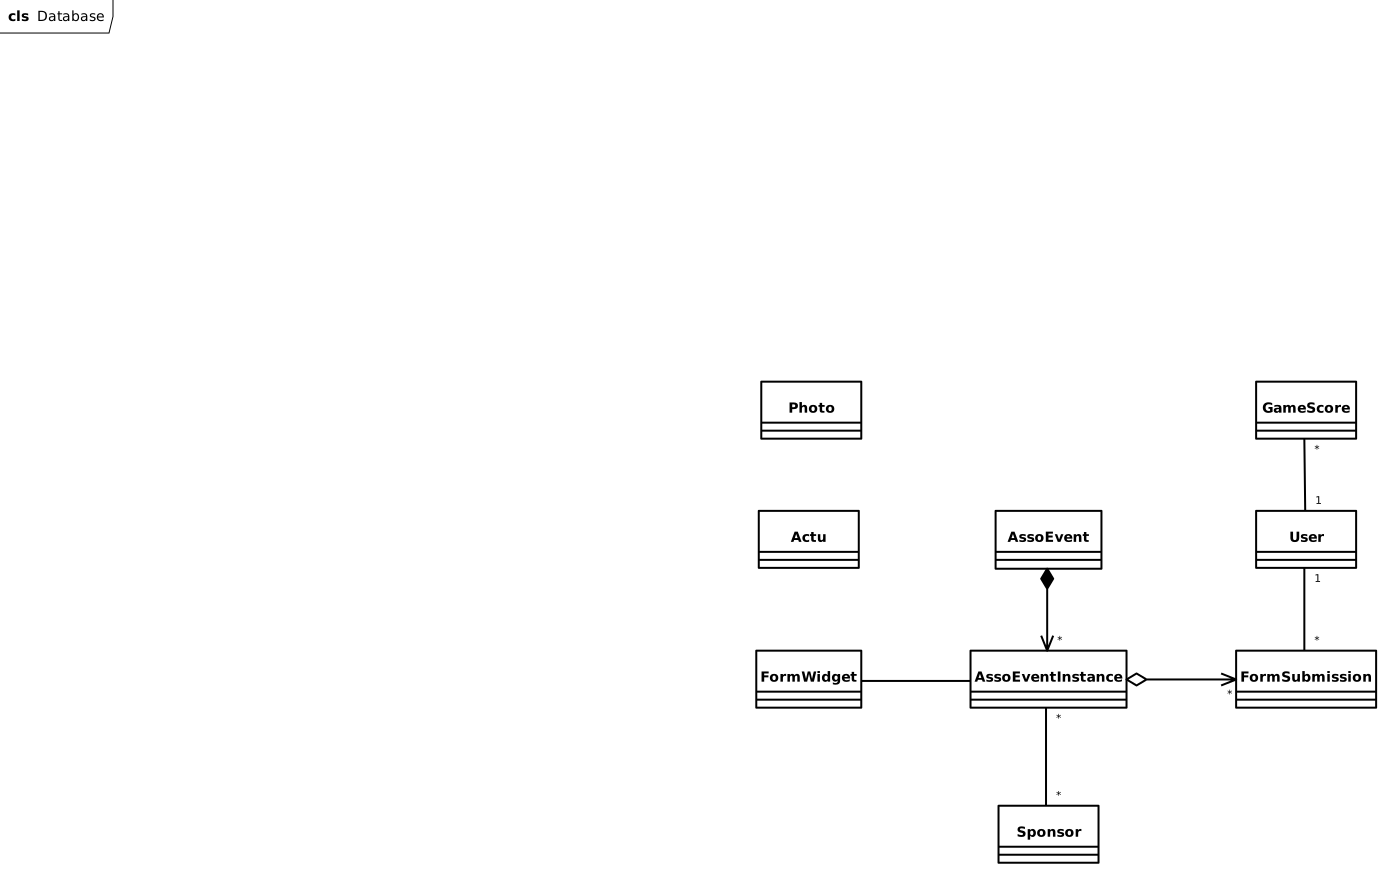
\includegraphics[width=\textwidth]{assets/pictures/database.png}
    \caption{Structure simplifiée de la base de données}
    \label{anx:gantt}
\end{figure}

\vspace{\stretch{1}}

\chapter{Bibliographie}

\begin{itemize}
    \item\bibquote{Symfony Documentation}{Symfony SAS}{https://symfony.com/doc/current/index.html}
    \item\bibquote{Twig Documentation}{Symfony SAS}{https://twig.symfony.com/doc/3.x/}
    \item\bibquote{Doctrine Documentation}{Doctrine Community}{https://www.doctrine-project.org/projects/doctrine-orm/en/2.9/index.html}
    \item\bibquote{PHP Documentation}{The PHP Group}{https://www.php.net/docs.php}
\end{itemize}

\pagebreak
\thispagestyle{empty}
~
\bigskip
\bigskip
\bigskip
\bigskip

\Large{\textbf{Résumé}}\normalsize
\label{chap:abstract-fr}
\bigskip

Dans le cadre de notre troisième année de Licence Informatique au sein de l’\univ, nous avons mené un projet tutoré visant à refondre le site \web\ de l’association étudiant \logo{OFNI}. L’objectif était de concevoir et développer un site moderne, ergonomique et maintenable, tout en appliquant nos connaissances en développement \web.

Le site, intègre des fonctionnalités essentielles, telles qu’une gestion d’événements dynamique, un espace membre, une boutique en ligne et un mini-jeu, \game, visant à encourager la visite du site par les étudiants. Au cours du développement, nous avons rencontré des problématiques techniques et administratives, notamment en ce qui concerne l’authentification des utilisateurs et le respect de la vie privée, encadré par le \logo{RGPD}. Nous avons mis en place un système de gestion flexible des inscriptions et des événements, favorisant la réutilisation des données via une approche factorisée de la gestion de ces derniers.
\bigskip
\bigskip


% \noindent
\Large{\textbf{Abstract}}\normalsize
\label{chap:abstract-en}
\bigskip

As part of our third year in the Computer Science degree program at \univ, we carried out a supervised project aimed at redesigning the \web\ platform of the student association \logo{OFNI}. The objective was to design and develop a modern, ergonomic, and maintainable website while applying our knowledge in \web\ development.

The website includes essential features such as dynamic event management, a member space, an online store, and a mini-game, \game, designed to encourage students to visit the platform regularly. During the development, we encountered technical and administrative challenges, particularly regarding user authentication and privacy compliance, as mandated by the \logo{RGPD}. To address these issues, we implemented a flexible registration and event management system, enabling data reuse through a factorized approach.
\bigskip
\bigskip


% \noindent
\large{\textbf{Mots-clés}}\normalsize
\bigskip


\noindent Développement web --- Automatisation --- Symfony --- JavaScript --- Sass --- RGPD --- Association
\bigskip
\bigskip

% \noindent
\large{\textbf{Keywords}}\normalsize
\bigskip



\noindent Web development --- Automation --- Symfony --- JavaScript --- Sass --- RGPD --- Association


\end{document}
